\section{Lecture 4}
\begin{tabular}{p{4cm}p{15cm}}
Resting potential	& Due to concentration differences, caused by a selectively permeable membrane, there is a permanent voltage difference between the interior and the exterior of a neuron. The resting potential can be computed by the GHK equation, which depends on the conductances (permeability in the biological context) of the membrane w.r.t. each ion.\\
Conductance		& The conductance of a membrane is determined by the ion channels of the membrane. The permeability of the ion channel is not constant. Instead, there are ligand-gated, strech-activated, light-gated (mostly synthesized) and voltage-gated ion channels. Therefore, the conductance of a membrane w.r.t. an ion $X$ is not constant. Voltage-gated ion channels depend on the membrane potential. They give rise to positive feedback loops (see below) and are capable to trigger action potentials. That's why we want to look at voltage-gated ion channels. So, the conductance depends on the voltage and a certain time constant, i.e. $g_X = g_X(V,\tau_X)$\\
Action potential	& Since the conductances for different ions change not equally fast, the potential difference can vary from the resting potential. Typically, the potential rises sharply, then falls again, undershoots and levels out again at the resting potential. This process is called an action potential.\\
Threshold potential	& The threshold potential is the level which must be reached for an action potential to be triggered.\\
			& 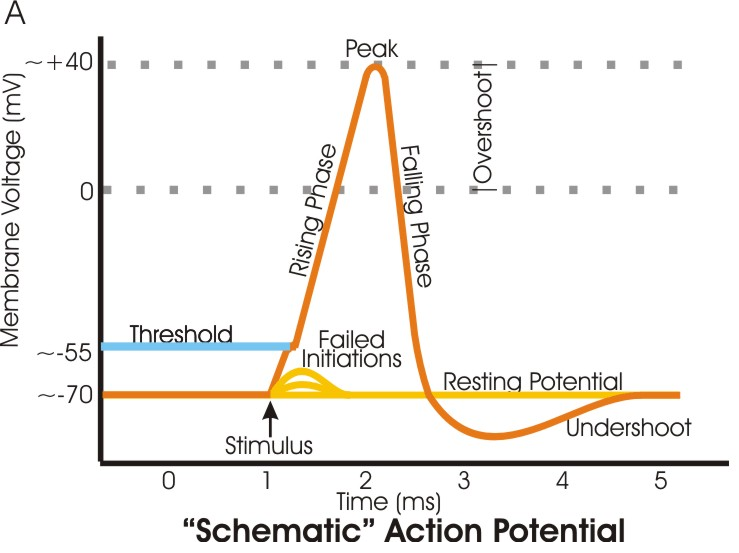
\includegraphics[width=12cm]{neuroinf_actionpotential.png}\\
\end{tabular}
\begin{longtable}{p{4cm}p{15cm}}
Membrane model	& 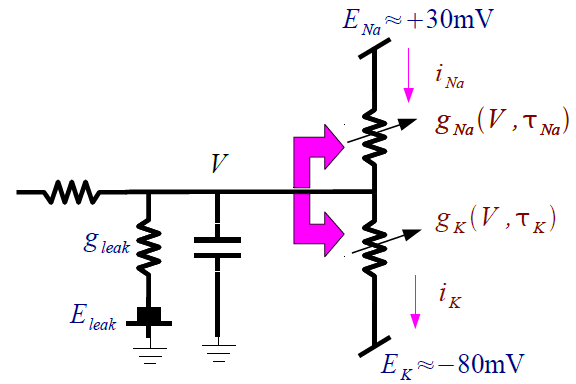
\includegraphics[width = 10cm]{neuroinf_membrane_as_circuit2.png}\\
		& The arrows indicate that the conductances depend on the voltage $V$. The capacitance is well-known, the subscript leak refers to the axon leakage and the resistance at the left refers to some dendrites or whatever.\\
Conductances w.r.t. Na$^+$ and K$^+$	& 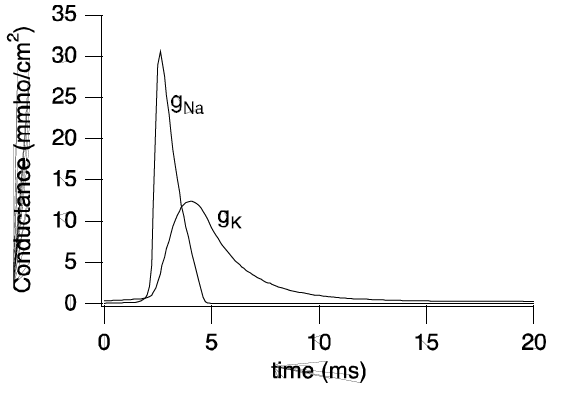
\includegraphics[width=8cm]{neuroinf_conductances.png}\\
Feedback loops	& If, for some reason (e.g. spike from other neuron), the membrane voltage increases (or decreases), the conductance for ion X rises (or falls) as well. This causes the X current to rise, which causes the membrane voltage to rise aka \textit{depolarization} (or fall aka \textit{hyperpolarization}) further and this causes the conductance to rise (or fall) further, resulting in a positive (or negative) feedback loop.\\
Action potential mechanism	& $\tau_{Na} < \tau_{K}$, that is, Sodium ions reacts faster on a voltage change than Potassium ions.\newline
		  If the membrane voltage change exceeds the threshold voltage, a \textit{positive feedback loop} w.r.t. Na$^+$ starts and Sodium ions enter.\newline
		  When Potassium reacts to the initial voltage change, the positive feedback loop ends and a \textit{negative feedback loop} w.r.t. K$^+$ starts and Potassium ions begin to leave the membrane. At this moment the maximal membrane potential is achieved.\\
Threshold potential value	& In this model, the threshold potential value is at the voltage where the Na$^+$ and the K$^+$ \textit{current} are equal, i.e. $V(I_{Na^+} = I_{K^+})$, because $\frac{dV}{dt}~ \propto ~ I$ and the feedback loop is about the increase or decrease, i.e. the \textit{change} in voltage.\\
Charge carriers	      & During the action potential, Sodium ions enter and Potassium ions leave the membrane. Hence, at the end of an action potential, the Na$^+$ and K$^+$ concentratios have changed. To restore the original ratio of ion concentrations, the ions are pumped back by the sodium potassium pump. This is a feasible task, since relatively few ions need to cross the membrane for the membrane voltage to change drastically.\\
Myelin	& Some axons are encapsulated by myelin, which is essentially a insulator $\Rightarrow \lambda$ becomes bigger! On the downside, it requires more space and myelinated regions cannot produce action potentials.\\
Ranvier-nodes	& Axons are not myelinated along their full length. Instead, regularly spaced unmyelinated patches, called the nodes of Ranvier, generate action potentials to reinforce the signal.\\
Termination	& Generally, the action potential ends in an axon terminal, where it leads to the release of neurotransmitters into the synaptic cleft. In addition, action potentials can also backpropagate into the dendrites.
\end{longtable}
\subsection{Hodgkin-Huxley equation}
In general, the Hodgkin-Huxley equation is again an equation which describes the membrane potential. Precisely, it describes the membrane voltage during the action potential by imposing time-dependent expressions for the conductances by a fit to experimental data.\\
\begin{tabular}{p{4cm}p{15cm}}
General form		& $C \frac{dV}{dt} + \bar{g}_K(V-E_K) + \bar{g}_{Na}(V-E_{Na} + \underbrace{\bar{g}_L (V-V_L)}_{generic leak} + I_{inj} = 0$\\
			& $\bar{g}_K = g_K n^4(t)\quad n(t) \in [0,1]$\\
			& $\bar{g}_{Na} = g_{Na} m^3(t)h(t)\quad m(t),h(t) \in [0,1]$\\
Fitting to experimental data	\\
- Potassium	& 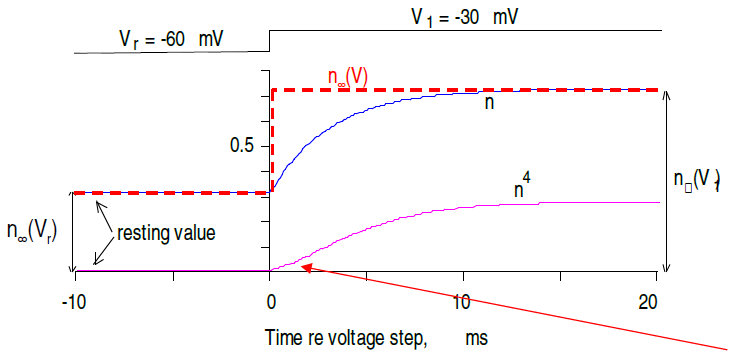
\includegraphics[width = 10cm]{neuroinf_hhm_n.png}\\
		& $g_K = \bar{g}_Kn^4$\\
- Sodium	& 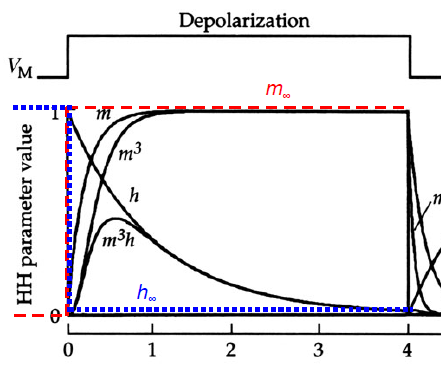
\includegraphics[width = 10cm]{neuroinf_hhm_mh.png}\\
		& $g_{Na} = \bar{g}_{Na} m^3h$
\end{tabular}

